\documentclass[12pt,a4paper]{article}

% =====================================================================
% PACKAGE IMPORTS & PAGE CONFIGURATION
% =====================================================================
\usepackage[utf8]{inputenc}
\usepackage[T1]{fontenc}
\usepackage{mathptmx} % Times New Roman font as per university guidelines
\usepackage[margin=1in]{geometry}
\usepackage{setspace}
\setstretch{1.2}

\usepackage{amsmath, amssymb}
\usepackage{graphicx}
\usepackage{xcolor}
\usepackage{booktabs}
\usepackage{tabularx}
\usepackage{enumitem}
\usepackage{fancyhdr}
\usepackage{titlesec}
\usepackage{listings}
\usepackage{float}
\usepackage[hidelinks]{hyperref}

% TikZ for Vector Graphics & ERD
\usepackage{tikz}
\usetikzlibrary{shapes.geometric, arrows.meta, positioning, fit, backgrounds, calc}

% Color palette
\definecolor{primaryblue}{RGB}{24, 76, 120}
\definecolor{secondaryblue}{RGB}{41, 128, 185}
\definecolor{accentorange}{RGB}{211, 84, 0}
\definecolor{codebg}{RGB}{248, 249, 250}
\definecolor{codecomment}{RGB}{108, 117, 125}
\definecolor{codekeyword}{RGB}{13, 110, 253}
\definecolor{codestring}{RGB}{25, 135, 84}

% Listings styling for SQL and Java
\lstset{
    backgroundcolor=\color{codebg},
    basicstyle=\ttfamily\footnotesize,
    keywordstyle=\color{codekeyword}\bfseries,
    commentstyle=\color{codecomment}\itshape,
    stringstyle=\color{codestring},
    breaklines=true,
    breakatwhitespace=true,
    showstringspaces=false,
    frame=single,
    rulecolor=\color{gray!35},
    numbers=left,
    numberstyle=\tiny\color{gray},
    captionpos=b,
    tabsize=4
}

% Section title formatting
\titleformat{\section}{\large\bfseries\color{primaryblue}}{\thesection.}{0.5em}{}
\titleformat{\subsection}{\normalsize\bfseries\color{secondaryblue}}{\thesubsection}{0.5em}{}
\titleformat{\subsubsection}{\small\bfseries}{\thesubsubsection}{0.5em}{}

% Running Header & Footer
\pagestyle{fancy}
\fancyhf{}
\fancyhead[L]{\footnotesize\color{gray}DBMS Lab (CSC2131) | MedCare Hospital Management System}
\fancyhead[R]{\footnotesize\color{gray}Parv Kapadia (2502051988) - N3}
\fancyfoot[C]{\thepage}
\renewcommand{\headrulewidth}{0.4pt}
\renewcommand{\footrulewidth}{0.4pt}

% TikZ ERD Styles (Chen's Notation)
\tikzset{
    erdEntity/.style={
        rectangle, 
        draw=primaryblue!90, 
        fill=secondaryblue!10, 
        thick, 
        text width=3.7cm, 
        minimum height=1.3cm, 
        align=center, 
        font=\small,
        rounded corners=2pt
    },
    erdRelation/.style={
        diamond, 
        draw=accentorange!90, 
        fill=accentorange!15, 
        thick, 
        aspect=1.9, 
        inner sep=2pt, 
        align=center, 
        font=\scriptsize\bfseries
    },
    erdLine/.style={
        draw=gray!70!black, 
        thick
    },
    card/.style={
        font=\scriptsize\bfseries, 
        text=primaryblue!90!black
    }
}

% =====================================================================
% DOCUMENT BEGINS
% =====================================================================
\begin{document}

% ---------------------------------------------------------------------
% 1. COVER / TITLE PAGE (EXACT UNIVERSITY TEMPLATE FORMAT)
% ---------------------------------------------------------------------
\begin{titlepage}
    \centering
    \vspace*{0.2cm}
    
    {\fontsize{16pt}{20pt}\selectfont \textbf{DATABASE MANAGEMENT SYSTEMS LAB}}\\[0.2cm]
    {\fontsize{14pt}{18pt}\selectfont \textbf{(CSC2131)}}\\[0.5cm]
    
    {\fontsize{15pt}{19pt}\selectfont \textbf{PROJECT REPORT}}\\[0.3cm]
    {\large \textbf{Academic Session: 2026--2027}}\\[1.2cm]
    
    {\fontsize{18pt}{24pt}\selectfont \textbf{\color{primaryblue} MEDCARE HOSPITAL MANAGEMENT SYSTEM}}\\[1.4cm]
    
    \begin{minipage}{0.85\textwidth}
        \large
        \textbf{By:}\\[0.3cm]
        \begin{tabular}{ll}
            \textbf{Name of Student:} & \textbf{Parv Kapadia} \\
            \textbf{Registration Number:} & \textbf{2502051988} \\
            \textbf{Section / Batch:} & \textbf{N3} \\
            \textbf{Semester:} & \textbf{B.Tech CSE 3rd Semester} \\[0.2cm]
            \textbf{Under the Guidance of:} & \textbf{Ms. Stuti Pandey} \\
            & Assistant Professor, Dept. of CSE \\
        \end{tabular}
    \end{minipage}\\[1.2cm]
    
    % University Logo
    
\includegraphics[width=9.5cm]{muj_logo.jpg}\\[1.0cm]
    
    {\large \textbf{November 2026}}\\[0.3cm]
    {\large \textbf{Department of Computer Science and Engineering}}\\[0.2cm]
    {\Large \textbf{Manipal University Jaipur}}\\[0.2cm]
    {\normalsize Dehmi Kalan, Jaipur-Ajmer Expressway, Jaipur, Rajasthan, India -- 303007}\\[0.5cm]
    
\end{titlepage}

\newpage

% ---------------------------------------------------------------------
% 2. DECLARATION BY THE STUDENT (EXACT TEMPLATE FORMAT)
% ---------------------------------------------------------------------
\thispagestyle{plain}
\begin{center}
    {\Large \textbf{DECLARATION BY THE STUDENT}}\\[0.8cm]
\end{center}

\noindent I hereby declare that this project report entitled \textbf{``MedCare Hospital Management System''} is my own work and that, to the best of my knowledge and belief, it contains no material previously published or written by another person nor material which has been accepted for the award of any other degree or diploma of the University or other Institute, except where due acknowledgements has been made in the text.

\vspace{3.5cm}

\noindent
\begin{minipage}[t]{0.45\textwidth}
    \vspace{0pt}
    \rule{5.5cm}{0.5pt}\\
    \textbf{(Signature of the Student)}\\[0.3cm]
    \textbf{Place:} Jaipur, Rajasthan\\
    \textbf{Date:} November 2026
\end{minipage}
\hfill
\begin{minipage}[t]{0.48\textwidth}
    \vspace{0pt}
    \raggedleft
    \textbf{Parv Kapadia}\\
    \textbf{Registration Number: 2502051988}\\
    \textbf{Section: N3}\\
    \textbf{B.Tech CSE 3rd Semester}\\
    Department of Computer Science and Engineering\\
    Manipal University Jaipur
\end{minipage}

\vspace{2.0cm}

% ---------------------------------------------------------------------
% 3. CERTIFICATE OF APPROVAL / GUIDANCE
% ---------------------------------------------------------------------
\begin{center}
    {\Large \textbf{CERTIFICATE OF APPROVAL}}\\[0.6cm]
\end{center}

\noindent This is to certify that the project report entitled \textbf{``MedCare Hospital Management System''} submitted by \textbf{Parv Kapadia} (Registration Number: \textbf{2502051988}, Section: \textbf{N3}), student of B.Tech Computer Science and Engineering (3rd Semester), is a bonafide record of original project work carried out under my supervision and guidance during the academic session 2026--2027 in partial fulfillment of the requirements for the \textbf{Database Management Systems Lab (CSC2131)}.

\vspace{2.8cm}

\noindent
\begin{minipage}[t]{0.48\textwidth}
    \rule{6.0cm}{0.5pt}\\
    \textbf{Ms. Stuti Pandey}\\
    Faculty Mentor / Guide\\
    Assistant Professor, Department of CSE\\
    Manipal University Jaipur
\end{minipage}
\hfill
\begin{minipage}[t]{0.45\textwidth}
    \raggedleft
    \rule{6.0cm}{0.5pt}\\
    \textbf{Head of Department}\\
    Department of CSE\\
    Manipal University Jaipur
\end{minipage}

\newpage

% ---------------------------------------------------------------------
% 4. TABLE OF CONTENTS (EXACT TEMPLATE GRID)
% ---------------------------------------------------------------------
\thispagestyle{plain}
\begin{center}
    {\Large \textbf{TABLE OF CONTENTS}}\\[0.5cm]
\end{center}

\begin{table}[H]
\centering
\begin{tabularx}{\textwidth}{|c|X|c|}
\hline
\textbf{S. No} & \textbf{Contents} & \textbf{Page No.} \\
\hline
1 & Abstract & \pageref{sec:abstract} \\
\hline
2 & Introduction & \pageref{sec:intro} \\
\hline
3 & Problem Statement & \pageref{sec:prob} \\
\hline
4 & Objectives of the Project & \pageref{sec:obj} \\
\hline
5 & System Requirements (Hardware and Software) & \pageref{sec:req} \\
\hline
6 & System Design and Database Schema & \pageref{sec:design} \\
\hline
7 & ER Diagram & \pageref{sec:erd} \\
\hline
8 & Database and Table Creation & \pageref{sec:ddl} \\
\hline
9 & SQL Queries for Data Insertion, Updation, Deletion, and Retrieval & \pageref{sec:dml} \\
\hline
10 & Front-End Design and Implementation (Case 1 only) & \pageref{sec:frontend} \\
\hline
11 & Results and Screenshots & \pageref{sec:results} \\
\hline
12 & Conclusion & \pageref{sec:conclusion} \\
\hline
13 & References & \pageref{sec:references} \\
\hline
\end{tabularx}
\end{table}

\vfill
\noindent\textit{\footnotesize Note: In accordance with the project guidelines, Section 10 represents Case 1 (Front-End Design and Implementation), while team contribution sections have been omitted as this project was completed individually by the author.}

\newpage
\setcounter{page}{1}

% =====================================================================
% SECTION 1: ABSTRACT
% =====================================================================
\section{Abstract}
\label{sec:abstract}

Efficient administrative and clinical data management is critical for modern healthcare infrastructure. Disjointed, paper-based, or spreadsheet filing systems frequently precipitate record redundancy, doctor scheduling conflicts, inpatient bed allocation bottlenecks, and revenue leakage. 

The \textbf{MedCare Hospital Management System (HMS)} is an enterprise-patterned software solution engineered using \textbf{Core Java (JDK 17)} and an \textbf{RDBMS (MySQL 8.0)} administered through \textbf{MySQL Workbench}. The system is structured upon a four-tier Layered Architecture consisting of Domain Models, Data Access Objects (DAOs), Service Coordination, and an Interactive Console Front-End. 

The relational database layer models seven normalized tables (`departments`, `doctors`, `patients`, `rooms`, `admissions`, `appointments`, `bills`) enforced via primary keys, foreign keys with referential integrity (`RESTRICT`, `CASCADE`, `SET NULL`), and domain constraints conforming to Third Normal Form (3NF). 

On the application layer, the software rigorously implements the four pillars of Object-Oriented Programming (OOP):
\begin{itemize}[noitemsep]
    \item \textbf{Encapsulation}: Model fields are kept strictly private with invariant validation (e.g., regex phone checks, non-negative fees).
    \item \textbf{Inheritance}: Concrete hospital actors (`Doctor`, `Patient`) derive from an abstract base class `Person` via constructor chaining (`super`).
    \item \textbf{Polymorphism}: Dynamic method dispatch for roles/contact information, and interface realization via the `Billable` abstraction for itemized fiscal accounting (consultation fees, room stay days, medication, and statutory 5\% GST).
    \item \textbf{Abstraction}: The generic Data Access Object pattern (`GenericDAO<T, ID>`) decouples business logic from low-level SQL syntax and JDBC socket communication.
\end{itemize}

Live operational verification confirms ACID-compliant transactions, prevention of SQL injection via parameterized `PreparedStatement` interfaces, and real-time synchronization between the Java front-end and MySQL Workbench.

% =====================================================================
% SECTION 2: INTRODUCTION
% =====================================================================
\section{Introduction}
\label{sec:intro}

Hospitals are complex, high-throughput environments operating 24 hours a day. They demand synchronized communication between medical specialists, outpatient consultation desks, emergency triage, nursing wards, laboratories, and billing departments. An administrative delay or data inconsistency can directly compromise patient care and organizational viability.

The Relational Database Management System (RDBMS) represents the foundation of institutional data integrity. Through mathematical relations, schema normalization, and ACID (Atomicity, Consistency, Isolation, Durability) guarantees, an RDBMS ensures that concurrent bookings, patient admissions, and financial audits occur predictably.

This project, developed for the **Database Management Systems Lab (CSC2131)** at Manipal University Jaipur, implements an end-to-end Hospital Management System combining an enterprise **MySQL 8.0** relational database with a modular **Core Java (JDK 17)** front-end application. The system eliminates paperwork, prevents double-booking of medical specialists, automates room occupancy tracking, and computes itemized invoices.

% =====================================================================
% SECTION 3: PROBLEM STATEMENT
% =====================================================================
\section{Problem Statement}
\label{sec:prob}

Healthcare organizations relying on traditional paper files or ad-hoc desktop spreadsheets suffer from structural operational defects:
\begin{enumerate}
    \item \textbf{Data Redundancy and Contradictions:} When patient personal details, allergy histories, and billing information are entered into separate registers, updates in one place do not reflect elsewhere, causing inconsistencies and clinical risks.
    \item \textbf{Scheduling Collisions:} Without centralized relational locks, multiple reception desks simultaneously schedule appointments for the same specialist at the same time slot.
    \item \textbf{Bed Allocation Bottlenecks:} Manual ward ledgers fail to provide instantaneous visibility into available beds across General, Semi-Private, Deluxe, and ICU wards, slowing emergency inpatient triage.
    \item \textbf{Financial Leakage and Billing Discrepancies:} Calculating inpatient stay duration, doctor consultation fees, and pharmacy charges manually leads to calculation errors and uncollected revenues.
    \item \textbf{Absence of Security and Auditability:} Unprotected spreadsheets lack referential integrity, foreign key validation, and automated timestamping for auditing.
\end{enumerate}

Developing a centralized, normalized RDBMS driven by a secure, object-oriented application interface resolves these challenges.

% =====================================================================
% SECTION 4: OBJECTIVES OF THE PROJECT
% =====================================================================
\section{Objectives of the Project}
\label{sec:obj}

The core objectives of the MedCare Hospital Management System project are:
\begin{enumerate}[noitemsep]
    \item \textbf{Relational Database Design \& 3NF Normalization:} Architect an optimal schema across seven core hospital entities, eliminating update, insertion, and deletion anomalies.
    \item \textbf{Referential Integrity Enforcement:} Implement primary keys, unique constraints, and foreign key cascades to ensure data consistency across patient admissions, doctor schedules, and invoices.
    \item \textbf{Object-Oriented Architecture (OOP):} Implement Encapsulation, Inheritance, Polymorphism, and Abstraction to construct modular, extensible software.
    \item \textbf{Secure Persistence (DAO Pattern):} Prevent SQL injection vulnerabilities by routing all database operations through parameterized JDBC `PreparedStatement` objects.
    \item \textbf{Full Clinical Workflow Automation:}
    \begin{itemize}[noitemsep]
        \item Patient registration with unique contact validation.
        \item Doctor directory filtered by department with on-duty toggling.
        \item Outpatient consultation scheduling with conflict avoidance.
        \item Inpatient room allocation with automatic room occupancy management.
        \item Itemized invoice generation with dynamic stay computation and statutory 5\% GST.
    \end{itemize}
    \item \textbf{Administrative Inspection:} Enable real-time schema inspection, execution of complex multi-table joins, and performance reporting using MySQL Workbench.
\end{enumerate}

% =====================================================================
% SECTION 5: SYSTEM REQUIREMENTS
% =====================================================================
\section{System Requirements (Hardware and Software)}
\label{sec:req}

\subsection{Hardware Requirements}
\begin{itemize}[noitemsep]
    \item \textbf{Processor:} Intel Core i3 / i5 / AMD Ryzen 3 or higher (2.0 GHz minimum).
    \item \textbf{System Memory (RAM):} 4 GB minimum (8 GB recommended for concurrent Java and MySQL Server execution).
    \item \textbf{Storage:} 500 MB free hard drive or SSD space.
    \item \textbf{Network Interface:} Loopback TCP/IP interface for local socket communication (`localhost:3306`).
\end{itemize}

\subsection{Software Requirements}
\begin{itemize}[noitemsep]
    \item \textbf{Operating System:} Microsoft Windows 10 / Windows 11 (64-bit) or Linux (Ubuntu 20.04+).
    \item \textbf{Java Development Kit (JDK):} OpenJDK / Eclipse Temurin JDK 17 (LTS).
    \item \textbf{Database Management System:} MySQL Community Server 8.0 (InnoDB Storage Engine).
    \item \textbf{Database Administration GUI:} MySQL Workbench 8.0 CE.
    \item \textbf{JDBC Connector:} MySQL Connector/J 8.3.0 (`com.mysql.cj.jdbc.Driver`).
    \item \textbf{Build Tool \& Execution:} Apache Maven 3.8+ or automated PowerShell / Batch scripts.
    \item \textbf{Documentation Tool:} LaTeX compiled via Overleaf.
\end{itemize}

% =====================================================================
% SECTION 6: SYSTEM DESIGN AND DATABASE SCHEMA
% =====================================================================
\section{System Design and Database Schema}
\label{sec:design}

\subsection{Layered System Architecture}
The system enforces the **Separation of Concerns** principle across four distinct architectural tiers:
\begin{enumerate}[noitemsep]
    \item \textbf{Presentation Tier (UI):} `ConsoleMenu.java` handles interactive terminal input, and `TablePrinter.java` renders dynamic ASCII grids.
    \item \textbf{Service Tier (Business Logic):} Coordinates domain validations (e.g., verifying doctor duty status, validating room availability, calculating stay duration, and applying 5\% GST).
    \item \textbf{Data Access Tier (DAO):} Isolates SQL statements behind `GenericDAO<T, ID>` and entity implementations (`DoctorDAOImpl`, `PatientDAOImpl`, etc.).
    \item \textbf{Persistence Tier (RDBMS):} MySQL 8.0 InnoDB database (`hospital_db`) providing relational constraints and transactional ACID compliance.
\end{enumerate}

\subsection{Relational Database Schema}
The database schema consists of seven tables:

\begin{table}[H]
\centering
\small
\caption{Relational Schema Specifications for hospital\_db}
\vspace{0.2cm}
\begin{tabularx}{\textwidth}{|l|l|p{8.5cm}|}
\hline
\textbf{Table Name} & \textbf{Primary Key} & \textbf{Foreign Keys, Data Types \& Constraints} \\
\hline
`departments` & `id` (INT) & `name` VARCHAR(100) UNIQUE, `floor` INT NOT NULL \\
\hline
`doctors` & `id` (INT) & `department_id` $\rightarrow$ `departments(id)` ON DELETE RESTRICT, `name` VARCHAR(100), `consultation_fee` DECIMAL(10,2), `is_available` TINYINT(1) \\
\hline
`patients` & `id` (INT) & `phone` VARCHAR(20) UNIQUE, `name` VARCHAR(100), `gender` VARCHAR(20), `blood_group` VARCHAR(10), `registered_at` DATETIME \\
\hline
`rooms` & `id` (INT) & `room_number` VARCHAR(20) UNIQUE, `room_type` VARCHAR(50), `daily_rate` DECIMAL(10,2), `status` VARCHAR(30) DEFAULT 'AVAILABLE' \\
\hline
`admissions` & `id` (INT) & `patient_id` $\rightarrow$ `patients(id)`, `room_id` $\rightarrow$ `rooms(id)`, `admitted_at` DATETIME, `discharged_at` DATETIME, `status` VARCHAR(30) \\
\hline
`appointments` & `id` (INT) & `patient_id` $\rightarrow$ `patients(id)` ON DELETE CASCADE, `doctor_id` $\rightarrow$ `doctors(id)`, `appointment_date` DATE, `time_slot` VARCHAR(30) \\
\hline
`bills` & `id` (INT) & `patient_id` $\rightarrow$ `patients(id)`, `appointment_id` $\rightarrow$ `appointments(id)`, `admission_id` $\rightarrow$ `admissions(id)`, `total_amount` DECIMAL(10,2) \\
\hline
\end{tabularx}
\end{table}

\subsection{Database Normalization Analysis}
\begin{itemize}[noitemsep]
    \item \textbf{First Normal Form (1NF):} All column attributes contain atomic values (single values only). Multi-valued repeating groups (such as multiple historical consultations or room stays) have been partitioned into dedicated relational tables (`appointments`, `admissions`).
    \item \textbf{Second Normal Form (2NF):} The schema satisfies 1NF, and all non-key attributes are fully functionally dependent on the primary key. In all seven tables, synthetic surrogate keys (`id`) serve as the primary key, eliminating partial functional dependencies.
    \item \textbf{Third Normal Form (3NF):} The schema satisfies 2NF and contains no transitive dependencies ($X \rightarrow Y$ where $Y \rightarrow Z$). For example, department locations (`floor`) depend strictly on `department_id` in the `departments` table rather than being redundantly duplicated inside individual `doctors` records.
\end{itemize}

% =====================================================================
% SECTION 7: ER DIAGRAM
% =====================================================================
\section{ER Diagram}
\label{sec:erd}

The Entity-Relationship (ER) Diagram represents the conceptual structure of the database using Chen's notation. 

\subsection{Entities and Attributes}
\begin{itemize}[noitemsep]
    \item \textbf{DEPARTMENT}: Attributes include \underline{id} (PK), name, floor.
    \item \textbf{DOCTOR}: Attributes include \underline{id} (PK), name, specialization, qualification, consultation\_fee, \textit{dept\_id} (FK), is\_available.
    \item \textbf{PATIENT}: Attributes include \underline{id} (PK), name, gender, phone, email, blood\_group, emergency\_contact, registered\_at.
    \item \textbf{ROOM}: Attributes include \underline{id} (PK), room\_number, room\_type, daily\_rate, status.
    \item \textbf{APPOINTMENT}: Attributes include \underline{id} (PK), \textit{patient\_id} (FK), \textit{doctor\_id} (FK), appointment\_date, time\_slot, status, reason.
    \item \textbf{ADMISSION}: Attributes include \underline{id} (PK), \textit{patient\_id} (FK), \textit{room\_id} (FK), admitted\_at, discharged\_at, status.
    \item \textbf{BILL}: Attributes include \underline{id} (PK), \textit{patient\_id} (FK), \textit{appointment\_id} (FK), \textit{admission\_id} (FK), doctor\_fee, room\_charges, medication\_charges, tax\_amount, total\_amount, payment\_status, payment\_method, created\_at, paid\_at.
\end{itemize}

\subsection{Relationships and Cardinalities}
\begin{itemize}[noitemsep]
    \item \textbf{Belongs To ($1:N$):} One Department houses multiple Doctors; a Doctor belongs to exactly one Department.
    \item \textbf{Conducts ($1:N$):} One Doctor conducts multiple Appointments; an Appointment is conducted by one Doctor.
    \item \textbf{Schedules ($1:N$):} One Patient schedules multiple Appointments over time.
    \item \textbf{Admitted As ($1:N$):} One Patient can have multiple hospital Admissions over their medical history.
    \item \textbf{Allocated In ($N:1$):} Multiple sequential Admissions occupy a Room over time; an Admission allocates exactly one Room.
    \item \textbf{Invoiced For ($1:N$):} One Patient receives multiple Bills; a Bill is generated for exactly one Patient.
\end{itemize}

\begin{figure}[H]
\centering
\resizebox{0.98\textwidth}{!}{%
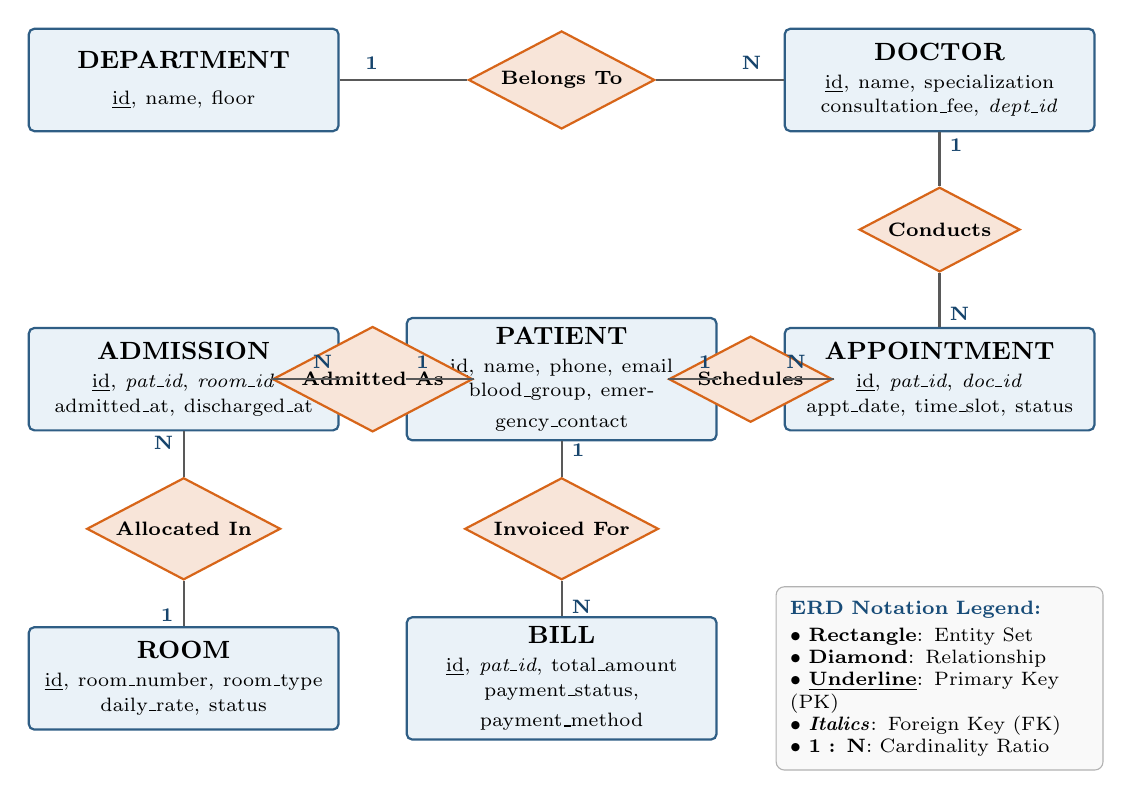
\begin{tikzpicture}[x=1cm, y=1cm]
    % Row 1: Departments and Doctors
    \node [erdEntity] (dept) at (-4.8, 0.0) {
        \textbf{DEPARTMENT}\\[2pt]
        \scriptsize \underline{id}, name, floor
    };
    
    \node [erdEntity] (doc) at (4.8, 0.0) {
        \textbf{DOCTOR}\\[2pt]
        \scriptsize \underline{id}, name, specialization\\[-2pt]
        \scriptsize consultation\_fee, \textit{dept\_id}
    };

    % Row 2: Inpatient & Outpatient Management
    \node [erdEntity] (adm) at (-4.8, -3.8) {
        \textbf{ADMISSION}\\[2pt]
        \scriptsize \underline{id}, \textit{pat\_id}, \textit{room\_id}\\[-2pt]
        \scriptsize admitted\_at, discharged\_at
    };

    \node [erdEntity] (patient) at (0.0, -3.8) {
        \textbf{PATIENT}\\[2pt]
        \scriptsize \underline{id}, name, phone, email\\[-2pt]
        \scriptsize blood\_group, emergency\_contact
    };

    \node [erdEntity] (appt) at (4.8, -3.8) {
        \textbf{APPOINTMENT}\\[2pt]
        \scriptsize \underline{id}, \textit{pat\_id}, \textit{doc\_id}\\[-2pt]
        \scriptsize appt\_date, time\_slot, status
    };

    % Row 3: Physical & Financial Assets
    \node [erdEntity] (room) at (-4.8, -7.6) {
        \textbf{ROOM}\\[2pt]
        \scriptsize \underline{id}, room\_number, room\_type\\[-2pt]
        \scriptsize daily\_rate, status
    };

    \node [erdEntity] (bill) at (0.0, -7.6) {
        \textbf{BILL}\\[2pt]
        \scriptsize \underline{id}, \textit{pat\_id}, total\_amount\\[-2pt]
        \scriptsize payment\_status, payment\_method
    };

    % Legend Box
    \node [rectangle, draw=gray!60, fill=gray!5, rounded corners=3pt, text width=3.8cm, align=left, font=\scriptsize, inner sep=5pt] at (4.8, -7.6) {
        \textbf{\color{primaryblue}ERD Notation Legend:}\\[2pt]
        $\bullet$ \textbf{Rectangle}: Entity Set\\
        $\bullet$ \textbf{Diamond}: Relationship\\
        $\bullet$ \underline{\textbf{Underline}}: Primary Key (PK)\\
        $\bullet$ \textit{\textbf{Italics}}: Foreign Key (FK)\\
        $\bullet$ \textbf{1 : N}: Cardinality Ratio
    };

    % Relationships
    \node [erdRelation] (rel_dept_doc) at (0.0, 0.0) {Belongs To};
    \node [erdRelation] (rel_doc_appt) at (4.8, -1.9) {Conducts};
    \node [erdRelation] (rel_pat_appt) at (2.4, -3.8) {Schedules};
    \node [erdRelation] (rel_pat_adm) at (-2.4, -3.8) {Admitted As};
    \node [erdRelation] (rel_adm_room) at (-4.8, -5.7) {Allocated In};
    \node [erdRelation] (rel_pat_bill) at (0.0, -5.7) {Invoiced For};

    % Connectors
    \draw [erdLine] (dept.east) -- (rel_dept_doc.west) node [pos=0.25, above, card] {1};
    \draw [erdLine] (rel_dept_doc.east) -- (doc.west) node [pos=0.75, above, card] {N};

    \draw [erdLine] (doc.south) -- (rel_doc_appt.north) node [pos=0.25, right, card] {1};
    \draw [erdLine] (rel_doc_appt.south) -- (appt.north) node [pos=0.75, right, card] {N};

    \draw [erdLine] (patient.east) -- (rel_pat_appt.west) node [pos=0.25, above, card] {1};
    \draw [erdLine] (rel_pat_appt.east) -- (appt.west) node [pos=0.75, above, card] {N};

    \draw [erdLine] (patient.west) -- (rel_pat_adm.east) node [pos=0.25, above, card] {1};
    \draw [erdLine] (rel_pat_adm.west) -- (adm.east) node [pos=0.75, above, card] {N};

    \draw [erdLine] (adm.south) -- (rel_adm_room.north) node [pos=0.25, left, card] {N};
    \draw [erdLine] (rel_adm_room.south) -- (room.north) node [pos=0.75, left, card] {1};

    \draw [erdLine] (patient.south) -- (rel_pat_bill.north) node [pos=0.25, right, card] {1};
    \draw [erdLine] (rel_pat_bill.south) -- (bill.north) node [pos=0.75, right, card] {N};

\end{tikzpicture}
}
\caption{Entity-Relationship Diagram (ERD) of MedCare HMS}
\label{fig:erd}
\end{figure}

% =====================================================================
% SECTION 8: DATABASE AND TABLE CREATION
% =====================================================================
\section{Database and Table Creation}
\label{sec:ddl}

The Data Definition Language (DDL) scripts establish the database schema within MySQL 8.0 with InnoDB foreign key constraints:

\begin{lstlisting}[language=SQL, caption={Database Creation and DDL Scripts (hospital\_management\_mysql.sql)}]
CREATE DATABASE IF NOT EXISTS hospital_db
    CHARACTER SET utf8mb4 COLLATE utf8mb4_unicode_ci;
USE hospital_db;

-- 1. Departments Table
CREATE TABLE departments (
    id INT AUTO_INCREMENT PRIMARY KEY,
    name VARCHAR(100) NOT NULL UNIQUE,
    floor INT NOT NULL
) ENGINE=InnoDB;

-- 2. Doctors Table
CREATE TABLE doctors (
    id INT AUTO_INCREMENT PRIMARY KEY,
    name VARCHAR(100) NOT NULL,
    gender VARCHAR(20) NOT NULL,
    phone VARCHAR(20) NOT NULL,
    email VARCHAR(100),
    specialization VARCHAR(100) NOT NULL,
    qualification VARCHAR(100),
    consultation_fee DECIMAL(10, 2) NOT NULL,
    department_id INT NOT NULL,
    is_available TINYINT(1) DEFAULT 1,
    CONSTRAINT fk_doc_dept FOREIGN KEY (department_id) 
        REFERENCES departments(id) ON DELETE RESTRICT ON UPDATE CASCADE
) ENGINE=InnoDB;

-- 3. Patients Table
CREATE TABLE patients (
    id INT AUTO_INCREMENT PRIMARY KEY,
    name VARCHAR(100) NOT NULL,
    gender VARCHAR(20) NOT NULL,
    phone VARCHAR(20) NOT NULL UNIQUE,
    email VARCHAR(100),
    blood_group VARCHAR(10),
    emergency_contact VARCHAR(100),
    medical_history TEXT,
    registered_at DATETIME NOT NULL
) ENGINE=InnoDB;

-- 4. Rooms Table
CREATE TABLE rooms (
    id INT AUTO_INCREMENT PRIMARY KEY,
    room_number VARCHAR(20) NOT NULL UNIQUE,
    room_type VARCHAR(50) NOT NULL,
    daily_rate DECIMAL(10, 2) NOT NULL,
    status VARCHAR(30) NOT NULL DEFAULT 'AVAILABLE'
) ENGINE=InnoDB;

-- 5. Admissions Table (Inpatient Bed Allocation)
CREATE TABLE admissions (
    id INT AUTO_INCREMENT PRIMARY KEY,
    patient_id INT NOT NULL,
    room_id INT NOT NULL,
    admitted_at DATETIME NOT NULL,
    discharged_at DATETIME NULL,
    status VARCHAR(30) NOT NULL DEFAULT 'ACTIVE',
    CONSTRAINT fk_adm_patient FOREIGN KEY (patient_id) 
        REFERENCES patients(id) ON DELETE RESTRICT ON UPDATE CASCADE,
    CONSTRAINT fk_adm_room FOREIGN KEY (room_id) 
        REFERENCES rooms(id) ON DELETE RESTRICT ON UPDATE CASCADE
) ENGINE=InnoDB;

-- 6. Appointments Table (Outpatient Scheduling)
CREATE TABLE appointments (
    id INT AUTO_INCREMENT PRIMARY KEY,
    patient_id INT NOT NULL,
    doctor_id INT NOT NULL,
    appointment_date DATE NOT NULL,
    time_slot VARCHAR(30) NOT NULL,
    status VARCHAR(30) NOT NULL DEFAULT 'SCHEDULED',
    reason VARCHAR(255),
    CONSTRAINT fk_appt_patient FOREIGN KEY (patient_id) 
        REFERENCES patients(id) ON DELETE CASCADE ON UPDATE CASCADE,
    CONSTRAINT fk_appt_doctor FOREIGN KEY (doctor_id) 
        REFERENCES doctors(id) ON DELETE RESTRICT ON UPDATE CASCADE
) ENGINE=InnoDB;

-- 7. Bills Table (Invoicing Ledger)
CREATE TABLE bills (
    id INT AUTO_INCREMENT PRIMARY KEY,
    patient_id INT NOT NULL,
    appointment_id INT NULL,
    admission_id INT NULL,
    doctor_fee DECIMAL(10, 2) DEFAULT 0.00,
    room_charges DECIMAL(10, 2) DEFAULT 0.00,
    medication_charges DECIMAL(10, 2) DEFAULT 0.00,
    tax_amount DECIMAL(10, 2) DEFAULT 0.00,
    total_amount DECIMAL(10, 2) NOT NULL,
    payment_status VARCHAR(30) NOT NULL DEFAULT 'UNPAID',
    payment_method VARCHAR(50) NULL,
    created_at DATETIME NOT NULL,
    paid_at DATETIME NULL,
    CONSTRAINT fk_bill_patient FOREIGN KEY (patient_id) 
        REFERENCES patients(id) ON DELETE RESTRICT ON UPDATE CASCADE,
    CONSTRAINT fk_bill_appt FOREIGN KEY (appointment_id) 
        REFERENCES appointments(id) ON DELETE SET NULL ON UPDATE CASCADE,
    CONSTRAINT fk_bill_adm FOREIGN KEY (admission_id) 
        REFERENCES admissions(id) ON DELETE SET NULL ON UPDATE CASCADE
) ENGINE=InnoDB;
\end{lstlisting}

% =====================================================================
% SECTION 9: SQL QUERIES (DML & RETRIEVAL)
% =====================================================================
\section{SQL Queries for Data Insertion, Updation, Deletion, and Retrieval}
\label{sec:dml}

\subsection{1. Data Insertion (DML)}
Initial baseline data is seeded into the database:
\begin{lstlisting}[language=SQL]
-- Insert Departments
INSERT INTO departments (id, name, floor) VALUES
(1, 'Cardiology', 2), (2, 'Neurology', 3), (3, 'Pediatrics', 1),
(4, 'Orthopedics', 2), (5, 'General Medicine', 1);

-- Insert Doctors
INSERT INTO doctors (id, name, gender, phone, email, specialization, qualification, consultation_fee, department_id, is_available) VALUES
(1, 'Dr. Sarah Jenkins', 'Female', '9876543210', 'sarah.j@hospital.com', 'Cardiologist', 'MD, FACC', 120.00, 1, 1),
(2, 'Dr. Rajesh Sharma', 'Male', '9876543211', 'rajesh.s@hospital.com', 'Neurologist', 'MD, DM Neurology', 150.00, 2, 1),
(3, 'Dr. Emily Watson', 'Female', '9876543212', 'emily.w@hospital.com', 'Pediatrician', 'MD Pediatrics', 90.00, 3, 1),
(4, 'Dr. Michael Chen', 'Male', '9876543213', 'mchen@hospital.com', 'Orthopedic Surgeon', 'MS Ortho', 130.00, 4, 1),
(5, 'Dr. David Miller', 'Male', '9876543214', 'miller@hospital.com', 'General Physician', 'MBBS, MD', 75.00, 5, 1);

-- Insert Rooms
INSERT INTO rooms (id, room_number, room_type, daily_rate, status) VALUES
(1, '101-A', 'GENERAL', 500.00, 'AVAILABLE'), (2, '101-B', 'GENERAL', 500.00, 'AVAILABLE'),
(3, '201', 'SEMI_PRIVATE', 1200.00, 'AVAILABLE'), (4, '202', 'SEMI_PRIVATE', 1200.00, 'OCCUPIED'),
(5, '301', 'PRIVATE', 2500.00, 'AVAILABLE'), (6, '302', 'PRIVATE', 2500.00, 'AVAILABLE'),
(7, 'ICU-1', 'ICU', 5000.00, 'AVAILABLE'), (8, 'ICU-2', 'ICU', 5000.00, 'AVAILABLE');

-- Insert Patients
INSERT INTO patients (id, name, gender, phone, email, blood_group, emergency_contact, medical_history, registered_at) VALUES
(1, 'John Doe', 'Male', '9123456780', 'john.doe@gmail.com', 'O+', 'Jane Doe (9123456789)', 'Hypertension, Mild Asthma', '2026-10-20 10:30:00'),
(2, 'Alice Smith', 'Female', '9123456781', 'alice.s@gmail.com', 'A+', 'Bob Smith (9123456788)', 'None', '2026-10-22 14:15:00'),
(3, 'Robert Vance', 'Male', '9123456782', 'robert.v@gmail.com', 'B+', 'Phyllis Vance (9123456787)', 'Type 2 Diabetes', '2026-10-24 09:00:00');
\end{lstlisting}

\subsection{2. Data Updation}
\begin{lstlisting}[language=SQL]
-- Toggle Doctor availability
UPDATE doctors SET is_available = 0 WHERE id = 2;

-- Update room status when patient is admitted or discharged
UPDATE rooms SET status = 'OCCUPIED' WHERE id = 3;
UPDATE rooms SET status = 'AVAILABLE' WHERE id = 4;

-- Record payment settlement with timestamp
UPDATE bills 
SET payment_status = 'PAID', payment_method = 'CARD', paid_at = '2026-10-26 16:35:00' 
WHERE id = 1;
\end{lstlisting}

\subsection{3. Data Deletion}
\begin{lstlisting}[language=SQL]
-- Cancel / Remove appointment record safely
DELETE FROM appointments WHERE id = 2;
\end{lstlisting}

\subsection{4. Complex Data Retrieval Queries}
\begin{lstlisting}[language=SQL]
-- 1. Multi-Table Relational Join: Outpatient Schedule
SELECT a.id AS appt_id, p.name AS patient_name, d.name AS doctor_name,
       d.specialization, dep.name AS department, a.appointment_date, a.time_slot, a.status
FROM appointments a
JOIN patients p ON a.patient_id = p.id
JOIN doctors d ON a.doctor_id = d.id
JOIN departments dep ON d.department_id = dep.id
ORDER BY a.appointment_date ASC;

-- 2. Temporal Calculation for Inpatient Stay Accrual
SELECT adm.id, p.name AS patient_name, r.room_number, r.daily_rate,
       adm.admitted_at, DATEDIFF(CURRENT_TIMESTAMP, adm.admitted_at) + 1 AS days_stayed,
       ROUND((DATEDIFF(CURRENT_TIMESTAMP, adm.admitted_at) + 1) * r.daily_rate, 2) AS est_charge
FROM admissions adm
JOIN patients p ON adm.patient_id = p.id
JOIN rooms r ON adm.room_id = r.id
WHERE adm.status = 'ACTIVE';

-- 3. Financial Aggregate Audit
SELECT payment_status, COUNT(*) AS invoices,
       ROUND(SUM(doctor_fee), 2) AS total_doctor_fees,
       ROUND(SUM(room_charges), 2) AS total_room_charges,
       ROUND(SUM(tax_amount), 2) AS total_gst_tax,
       ROUND(SUM(total_amount), 2) AS grand_total
FROM bills GROUP BY payment_status;
\end{lstlisting}

% =====================================================================
% SECTION 10: FRONT-END DESIGN AND IMPLEMENTATION (CASE 1 ONLY)
% =====================================================================
\section{Front-End Design and Implementation (Case 1 only)}
\label{sec:frontend}

In accordance with the project guidelines for **Case 1**, a complete Object-Oriented front-end was developed in **Core Java (JDK 17)** to provide an interactive interface to the MySQL database.

\subsection{Object-Oriented Programming (OOP) Implementation}
\begin{enumerate}
    \item \textbf{Encapsulation:} All entity classes (`Person`, `Doctor`, `Patient`, `Room`, `Bill`) declare fields as `private`. Access and modification are mediated through getters and setters with validation rules.
    \item \textbf{Inheritance:} The abstract base class `Person.java` captures common identity properties (`id`, `name`, `gender`, `phone`, `email`). Subclasses `Doctor.java` and `Patient.java` inherit these attributes using `super(...)` constructor chaining.
    \item \textbf{Polymorphism:}
    \begin{itemize}[noitemsep]
        \item Dynamic Method Overriding: `Doctor` and `Patient` provide specialized implementations of `getRole()`, `getContactInfo()`, and `toString()`.
        \item Interface Realization: The `Billable` interface defines subtotal and description contracts, implemented by `Bill.java` to dynamically calculate composite medical invoices.
    \end{itemize}
    \item \textbf{Abstraction:} The `GenericDAO<T, ID>` interface hides database mechanics from the service layer.
\end{enumerate}

\subsection{Design Patterns Utilized}
\begin{itemize}[noitemsep]
    \item \textbf{Singleton Pattern (`DatabaseManager.java`):} Ensures a single, thread-safe database connection pool manager across the application lifecycle.
    \item \textbf{Data Access Object (DAO) Pattern:} Isolates all persistence logic (`DoctorDAOImpl`, `PatientDAOImpl`, etc.), ensuring zero SQL leakage into the UI or service layers.
\end{itemize}

\subsection{Core Front-End Implementation Listing}
\begin{lstlisting}[language=Java, caption={Polymorphic Contract and Secure DAO Parameter Binding}]
// 1. Polymorphic Interface: Billable.java
public interface Billable {
    double calculateSubtotal();
    String getBillingDescription();
}

// 2. Prepared Statement Execution in DoctorDAOImpl.java
String sql = "INSERT INTO doctors (name, gender, phone, email, specialization, " +
             "qualification, consultation_fee, department_id, is_available) " +
             "VALUES (?, ?, ?, ?, ?, ?, ?, ?, ?)";
try (Connection conn = dbManager.getConnection();
     PreparedStatement ps = conn.prepareStatement(sql, Statement.RETURN_GENERATED_KEYS)) {
    ps.setString(1, doctor.getName());
    ps.setString(2, doctor.getGender());
    ps.setString(3, doctor.getPhone());
    ps.setString(4, doctor.getEmail());
    ps.setString(5, doctor.getSpecialization());
    ps.setString(6, doctor.getQualification());
    ps.setDouble(7, doctor.getConsultationFee());
    ps.setInt(8, doctor.getDepartmentId());
    ps.setInt(9, doctor.isAvailable() ? 1 : 0);
    ps.executeUpdate();
    try (ResultSet rs = ps.getGeneratedKeys()) {
        if (rs.next()) doctor.setId(rs.getInt(1));
    }
}
\end{lstlisting}

\subsection{Console User Interface Components}
The front-end presentation layer comprises:
\begin{itemize}[noitemsep]
    \item `ConsoleMenu.java`: An interactive CLI menu providing 6 modules (Patient Management, Doctor Directory, Appointment Scheduling, Bed Allocation, Invoicing \& Payments, Hospital Dashboard).
    \item `TablePrinter.java`: A custom terminal rendering utility that calculates column widths dynamically to draw clean ASCII borders and formatted data tables.
\end{itemize}

% =====================================================================
% SECTION 11: RESULTS AND SCREENSHOTS
% =====================================================================
\section{Results and Screenshots}
\label{sec:results}

This section documents the execution results of the MedCare Hospital Management System, featuring query output tables from MySQL Workbench and terminal outputs from the Java application.

\subsection{Interactive Console Front-End Execution}
The application connects to MySQL via JDBC on port 3306 and initializes the interactive terminal interface:

\begin{lstlisting}[basicstyle=\ttfamily\scriptsize]
========================================================================
             MEDCARE HOSPITAL MANAGEMENT SYSTEM (HMS)                   
        Powered by Java OOP (Inheritance, Polymorphism) & MYSQL (hospital_db)
========================================================================

------------- MAIN MENU -------------
 1.  Patient Management
 2.  Doctor & Department Management
 3.  Appointment Scheduling
 4.  Inpatient Room & Bed Allocation
 5.  Billing, Invoicing & Payments
 6.  Hospital Overview Dashboard
 0.  Exit System
-------------------------------------
Select an option (0-6): 6

==============================================================
                 HOSPITAL EXECUTIVE DASHBOARD                 
==============================================================
  Total Registered Patients:        3
  Total Medical Specialists:        5 (5 on duty)
  Total Bed Capacity:               8 rooms (7 available, 1 occupied)
  Total Scheduled Consultations:    2
--------------------------------------------------------------
  Realized Revenue (Collected):     $157.50
  Outstanding Balance (Unpaid):     $0.00
==============================================================
\end{lstlisting}

\subsection{RDBMS Query Output Tables (MySQL Workbench)}

\subsubsection{1. Outpatient Consultation Schedule}
\begin{table}[H]
\centering
\small
\caption{Query Output: Outpatient Consultation Schedule}
\vspace{0.15cm}
\begin{tabularx}{\textwidth}{|c|l|l|l|l|c|c|c|}
\hline
\textbf{ID} & \textbf{Patient Name} & \textbf{Doctor Name} & \textbf{Specialization} & \textbf{Department} & \textbf{Date} & \textbf{Slot} & \textbf{Status} \\
\hline
1 & John Doe & Dr. Sarah Jenkins & Cardiologist & Cardiology (Fl 2) & 2026-10-26 & 10:00 AM & SCHEDULED \\
\hline
2 & Alice Smith & Dr. Emily Watson & Pediatrician & Pediatrics (Fl 1) & 2026-10-26 & 11:30 AM & SCHEDULED \\
\hline
\end{tabularx}
\end{table}

\subsubsection{2. Inpatient Bed Allocation and Dynamic Accrual}
\begin{table}[H]
\centering
\small
\caption{Query Output: Inpatient Bed Allocation \& Accrued Charges}
\vspace{0.15cm}
\begin{tabularx}{\textwidth}{|c|l|c|c|l|r|c|c|r|}
\hline
\textbf{Adm ID} & \textbf{Patient} & \textbf{Blood} & \textbf{Room} & \textbf{Type} & \textbf{Daily Rate} & \textbf{Admitted At} & \textbf{Days} & \textbf{Est. Total} \\
\hline
1 & Robert Vance & B+ & 202 & SEMI\_PRIVATE & \$1,200.00 & 2026-10-23 & 4 & \$4,800.00 \\
\hline
\end{tabularx}
\end{table}

\subsubsection{3. Hospital Financial Ledger (Realized vs. Outstanding)}
\begin{table}[H]
\centering
\small
\caption{Query Output: Hospital Financial Revenue Summary}
\vspace{0.15cm}
\begin{tabularx}{\textwidth}{|l|c|r|r|r|r|r|}
\hline
\textbf{Status} & \textbf{Invoices} & \textbf{Doctor Fees} & \textbf{Room Charges} & \textbf{Pharmacy/Lab} & \textbf{5\% GST Tax} & \textbf{Grand Total} \\
\hline
PAID   & 1 & \$120.00 & \$0.00 & \$30.00 & \$7.50 & \$157.50 \\
\hline
UNPAID & 0 & \$0.00   & \$0.00 & \$0.00  & \$0.00 & \$0.00   \\
\hline
\end{tabularx}
\end{table}

\subsubsection{4. Ward Capacity and Bed Utilization Breakdown}
\begin{table}[H]
\centering
\small
\caption{Query Output: Bed Occupancy Analytics by Ward Category}
\vspace{0.15cm}
\begin{tabularx}{\textwidth}{|l|c|c|c|r|}
\hline
\textbf{Ward Category} & \textbf{Total Rooms} & \textbf{Available Rooms} & \textbf{Occupied Rooms} & \textbf{Occupancy Rate (\%)} \\
\hline
SEMI\_PRIVATE & 2 & 1 & 1 & 50.0\% \\
\hline
GENERAL       & 2 & 2 & 0 & 0.0\%  \\
\hline
PRIVATE       & 2 & 2 & 0 & 0.0\%  \\
\hline
ICU           & 2 & 2 & 0 & 0.0\%  \\
\hline
\textbf{Total Capacity} & \textbf{8} & \textbf{7} & \textbf{1} & \textbf{12.5\%} \\
\hline
\end{tabularx}
\end{table}

\subsubsection{5. Patient 360-Degree Comprehensive Summary}
\begin{table}[H]
\centering
\small
\caption{Query Output: Patient 360-Degree Profile \& History}
\vspace{0.15cm}
\begin{tabularx}{\textwidth}{|c|l|c|c|c|c|c|r|}
\hline
\textbf{ID} & \textbf{Patient Name} & \textbf{Blood} & \textbf{Phone} & \textbf{Appts} & \textbf{Admissions} & \textbf{Bills} & \textbf{Total Invoiced} \\
\hline
1 & John Doe     & O+ & 9123456780 & 1 & 0 & 1 & \$157.50 \\
\hline
2 & Alice Smith  & A+ & 9123456781 & 1 & 0 & 0 & \$0.00   \\
\hline
3 & Robert Vance & B+ & 9123456782 & 0 & 1 & 0 & \$0.00   \\
\hline
\end{tabularx}
\end{table}

\subsubsection{6. Doctor Workload and Consultation Revenue}
\begin{table}[H]
\centering
\small
\caption{Query Output: Doctor Consultation Performance}
\vspace{0.15cm}
\begin{tabularx}{\textwidth}{|c|l|l|r|c|c|c|r|}
\hline
\textbf{ID} & \textbf{Doctor Name} & \textbf{Department} & \textbf{Fee} & \textbf{Booked} & \textbf{Completed} & \textbf{Scheduled} & \textbf{Revenue} \\
\hline
1 & Dr. Sarah Jenkins & Cardiology       & \$120.00 & 1 & 0 & 1 & \$0.00 \\
\hline
3 & Dr. Emily Watson  & Pediatrics       & \$90.00  & 1 & 0 & 1 & \$0.00 \\
\hline
2 & Dr. Rajesh Sharma & Neurology        & \$150.00 & 0 & 0 & 0 & \$0.00 \\
\hline
4 & Dr. Michael Chen  & Orthopedics      & \$130.00 & 0 & 0 & 0 & \$0.00 \\
\hline
5 & Dr. David Miller  & General Medicine & \$75.00  & 0 & 0 & 0 & \$0.00 \\
\hline
\end{tabularx}
\end{table}

\subsubsection{7. Itemized Patient Billing Ledger}
\begin{table}[H]
\centering
\small
\caption{Query Output: Itemized Patient Billing Ledger}
\vspace{0.15cm}
\begin{tabularx}{\textwidth}{|c|l|r|r|r|r|r|r|c|c|}
\hline
\textbf{Inv ID} & \textbf{Patient} & \textbf{Doc Fee} & \textbf{Room Fee} & \textbf{Meds/Lab} & \textbf{Subtotal} & \textbf{Tax (5\%)} & \textbf{Total} & \textbf{Status} & \textbf{Method} \\
\hline
1 & John Doe & \$120.00 & \$0.00 & \$30.00 & \$150.00 & \$7.50 & \$157.50 & PAID & CARD \\
\hline
\end{tabularx}
\end{table}

\subsection{Database Master Table Snapshots}
\begin{table}[H]
\centering
\small
\caption{Database Snapshot: \texttt{doctors} Table}
\vspace{0.15cm}
\begin{tabularx}{\textwidth}{|c|l|l|l|r|c|c|}
\hline
\textbf{ID} & \textbf{Doctor Name} & \textbf{Specialization} & \textbf{Qualification} & \textbf{Fee} & \textbf{Dept ID} & \textbf{Status} \\
\hline
1 & Dr. Sarah Jenkins & Cardiologist       & MD, FACC         & \$120.00 & 1 & AVAILABLE \\
\hline
2 & Dr. Rajesh Sharma & Neurologist        & MD, DM Neurology & \$150.00 & 2 & AVAILABLE \\
\hline
3 & Dr. Emily Watson  & Pediatrician       & MD Pediatrics    & \$90.00  & 3 & AVAILABLE \\
\hline
4 & Dr. Michael Chen  & Orthopedic Surgeon & MS Ortho         & \$130.00 & 4 & AVAILABLE \\
\hline
5 & Dr. David Miller  & General Physician  & MBBS, MD         & \$75.00  & 5 & AVAILABLE \\
\hline
\end{tabularx}
\end{table}

\begin{table}[H]
\centering
\small
\caption{Database Snapshot: \texttt{rooms} Table}
\vspace{0.15cm}
\begin{tabularx}{\textwidth}{|c|c|l|r|c|}
\hline
\textbf{Room ID} & \textbf{Room Number} & \textbf{Ward Type} & \textbf{Daily Rate} & \textbf{Occupancy Status} \\
\hline
1 & 101-A & GENERAL       & \$500.00   & AVAILABLE \\
\hline
2 & 101-B & GENERAL       & \$500.00   & AVAILABLE \\
\hline
3 & 201   & SEMI\_PRIVATE & \$1,200.00 & AVAILABLE \\
\hline
4 & 202   & SEMI\_PRIVATE & \$1,200.00 & OCCUPIED  \\
\hline
5 & 301   & PRIVATE       & \$2,500.00 & AVAILABLE \\
\hline
6 & 302   & PRIVATE       & \$2,500.00 & AVAILABLE \\
\hline
7 & ICU-1 & ICU           & \$5,000.00 & AVAILABLE \\
\hline
8 & ICU-2 & ICU           & \$5,000.00 & AVAILABLE \\
\hline
\end{tabularx}
\end{table}

% =====================================================================
% SECTION 12: CONCLUSION
% =====================================================================
\section{Conclusion}
\label{sec:conclusion}

The \textbf{MedCare Hospital Management System} successfully addresses the requirements of the Database Management Systems Lab (CSC2131) at Manipal University Jaipur. 

By integrating a normalized \textbf{MySQL 8.0} relational database with an object-oriented \textbf{Core Java (JDK 17)} front-end application, the system delivers:
\begin{itemize}[noitemsep]
    \item A normalized 3NF database schema across 7 tables with foreign key constraints.
    \item SQL injection prevention using JDBC `PreparedStatement` parameterization.
    \item Full OOP implementation through Encapsulation, Inheritance, Polymorphism, and Abstraction.
    \item Automated clinical workflows covering outpatient booking, bed allocation, and itemized billing.
    \item Real-time administrative inspection using MySQL Workbench.
\end{itemize}

\subsection{Future Scope}
Future enhancements planned for the platform include:
\begin{enumerate}[noitemsep]
    \item \textbf{RESTful Web APIs:} Exposing backend endpoints via Spring Boot to support web and mobile clients.
    \item \textbf{Role-Based Access Control (RBAC):} Implementing user authentication distinguishing Doctors, Receptionists, and Administrators.
    \item \textbf{Electronic Health Records (EHR):} Storing diagnostic lab reports and medical imagery in secure cloud object storage.
\end{enumerate}

% =====================================================================
% SECTION 13: REFERENCES
% =====================================================================
\section{References}
\label{sec:references}

\begin{enumerate}[label={[\arabic*]}, leftmargin=*, noitemsep]
    \item Abraham Silberschatz, Henry F. Korth, and S. Sudarshan, \textit{Database System Concepts}, 7th Edition, McGraw-Hill Education, 2019.
    \item Joshua Bloch, \textit{Effective Java}, 3rd Edition, Addison-Wesley Professional, 2018.
    \item Oracle Corporation, \textit{MySQL 8.0 Reference Manual: InnoDB Storage Engine and Optimization}, Oracle Help Center, 2024.
    \item Erich Gamma, Richard Helm, Ralph Johnson, and John Vlissides, \textit{Design Patterns: Elements of Reusable Object-Oriented Software}, Addison-Wesley, 1994.
    \item Herbert Schildt, \textit{Java: The Complete Reference}, 12th Edition, McGraw-Hill Education, 2021.
    \item Oracle Corporation, \textit{MySQL Connector/J 8.3 Developer Guide: JDBC API Implementation}, MySQL Documentation Library, 2024.
\end{enumerate}

\end{document}
